\documentclass[12pt, twocolumn, letterpaper]{article}
\usepackage[a4paper, top=5em, bottom=3em, left=5em, right=5em ]{geometry}

\usepackage{graphicx}
\graphicspath{{images/}}



\title{ENT 331: \\
  Final Project Proposal}
\author{John Waczak}
\date{\today}


\begin{document}
\maketitle 

\section*{Pollinator}
I propose to study the Large Blue Butterfly (\textit{Maculinea  airon}). At first, I was attracted to this pollinator due to its powerful silhouette and striking blue color. After some brief research, though, I was fascinated to learn of this particular species' history. It was first identified in Britain more than two hundred years but as of the late 1970's was officially listed as extinct there. Recent conservation efforts have seen the butterfly resurface at 3 sites in Britain with good progress over the last half-decade. An image of the pollinator is shown below.

\begin{figure}[!hbt]
  \centering
  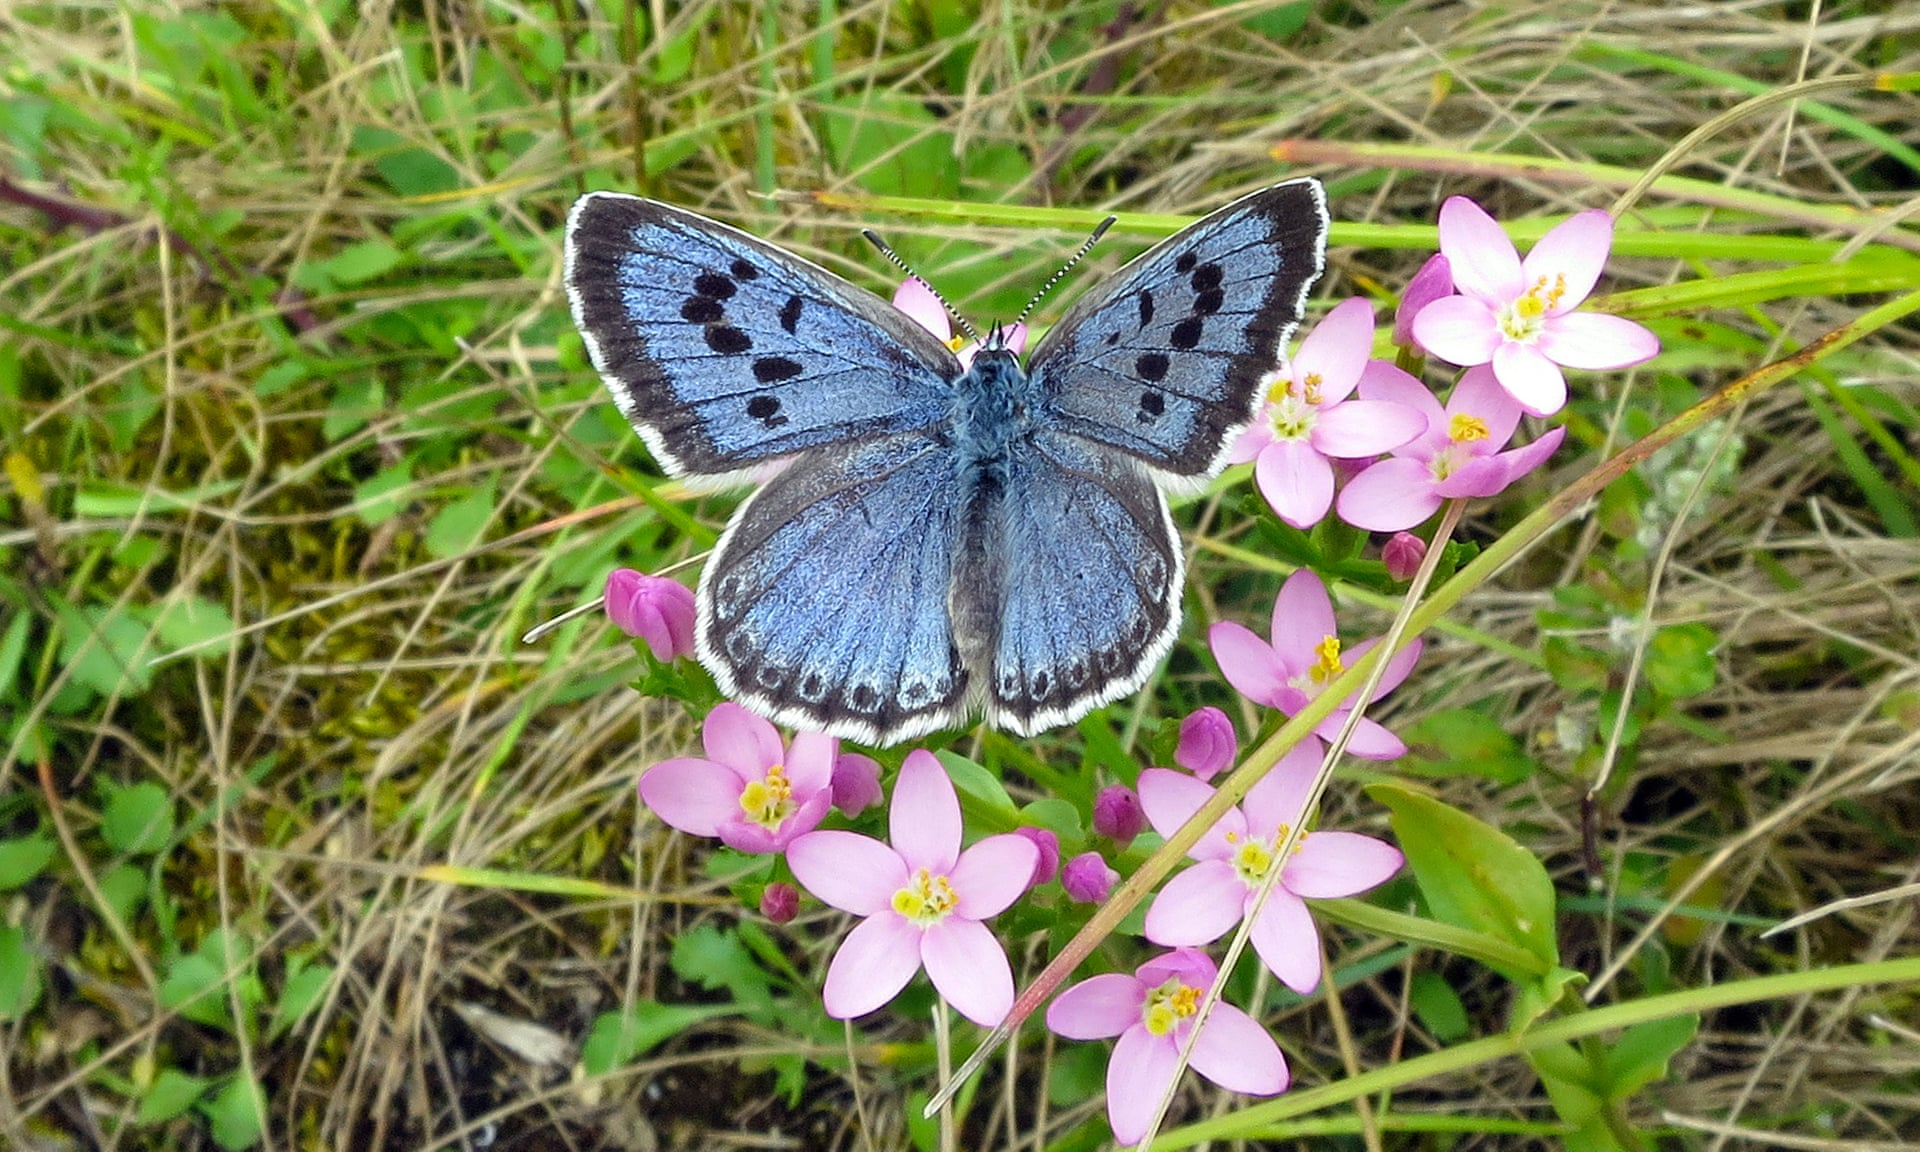
\includegraphics[width=1\columnwidth]{large_blue_1}
\end{figure}

\section*{Problem}
In the late 1900's, \textit{M. airon} began to experience a rapid decline in population that baffled scientists as the common sites where the butterfly was observed did not appear to have changed. Of the possibilities collection, insecticide use, and air pollution were suggested as culprits for the insect's disappearance.   \\

In my analysis I propose to address two key problems. The first is the lack of scientific understanding for the decline in population. The second problem is how to approach conservation efforts which have not been successful until recently. 

\section*{Solution}
As a solution to the first problem, I would like to perform a comprehensive literature review in order to analyze the following areas and their possible contribution to the decline of \textit{M. airon}:
\begin{enumerate}
\item \textbf{Pesticide use} The butterfly grows on short grasses laying it's eggs on thyme and other herbs. I would like to analyze the use of pesticides in these regions as well as this butterfly's LD50 for popular pesticides. 
\item \textbf{Collectors} One potential reason for the species' decline is collection. This pollinator is very unique among butterflies and is highly sought after for its unique color and speckling. 
\item \textbf{Habitat fragmentation and urabanization} One article I found suggests that the butterfly has only been successfully reintroduced to three sites. I imagine that urbanization in the UK may play in the decrease of habitat for \textit{M. airon}. 
\item \textbf{Mutualism dependencies} \textit{M. airon} is a specialist pollinator that has a close relationship with the few herbs (such as thyme) upon which it lays its eggs. It also shares an interesting parasitic relationship with Myrmica ant whose nests the \textit{M. airon} caterpillars predate upon. I am curious how these species are doing and whether or not they have experienced similar declines in this region.
\item \textbf{Climate Change} I would like to investigate the impact of climate change on the habitat of \textit{M. airon} and whether or not significant changes have occurred that may be affecting the pollinator.  

\end{enumerate}
Having analyzed these topics I should be able to summarize reasons for the butterfly's decline. \\

For the problem of reintroducing the species to its native habitat, I would
suggest that further land needs to be carefully cultivated if we desire to see
this butterfly repopulate. Those sites that have experienced some success have
cited tailor-made management of the land as the means to provide \textit{M.
  airon} enough support to survive. I would like to summarize historically
effective \textit{and} ineffective treatments for this particular problem. It
appears that the solution to this specie's problem rests with the careful
maintenance and cultivation of its habitat. \\

\noindent A list of sources I am planing to use can be found in the following
document.\\

\section*{General Outline}
I will follow the suggested format. The \textbf{Problem} I have identified is
the dying population of \textit{M. airon}. The \textbf{solution} to this problem as I see
it, which has already seen some success, is to carefully cultivate the habitat
of the pollinator by growing the necessary plants, allowing the right number of
animals to graze the area, and providing conditions to support the parasitic
host of the butterfly. The \textbf{key parties} are scientists researching the
cause of this species' collapse, citizens living near its habitat, and
conservation organizations. The \textbf{global context} is that this is one of
the first individual species to receive special conservation efforts and if we
can save this particular one, we will have demonstrated that humans can work to
save dying pollinators. 
\end{document}
